\section{Вычисление факториала}

\subsection{Условие задания}

Разработать приложение для вычисления факториала по приведенному примеру. 

Приложение должно содержать следующие компоненты:
\begin{enumerate}
    \item Заголовок формы должен отражать суть задания.
    \item Все элементы формы должны быть внятно подписаны (кнопки подписаны, у текстового поля должно быть написано, для чего оно нужно и т. д.)
    \item В коде должны быть комментарии и отступы (код должен быть легко читаем).
    \item В коде программы все элементы формы должны быть переименованы (btnName -  для кнопок, lblName - для ссылок, txtName - для текстового поля и т. д.) Наименования должны быть понятными.
    \item Приложение должно корректно работать (выводить ответ или ошибку с соответствующим сообщением) для следующих данных: ввод буквы, ввод отрицательного числа, ввод нуля, ввод положительного числа (< 10), ввод большого положительного числа. После вывода ошибок при вводе корректных данных поля ошибок должны очищаться.  
\end{enumerate}


\subsection{Вид формы в конструкторе}

Создано окно приложения, содержащее два элемента TextBox, два элемента
Label и один элемент Button. Вид окна представлен на рисунке \ref{task1_form} \cite{лаврентьев2020использование}. 

\begin{figure}[H]
    \centering
    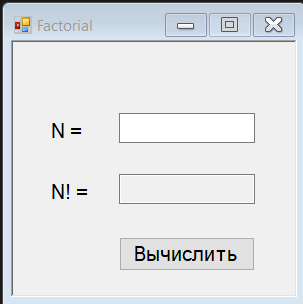
\includegraphics[width=0.3\linewidth]{lections/img/task1_form.png}
    \caption{Окно приложения <<factorial>> открытое в конструкторе }
    \label{task1_form}
\end{figure}


\subsection{Таблица с описанием переименованных элементов формы}
Все измененные элементы формы указаны в таблице \ref{task1_attributes}.
\begin{table}[H]
\caption{Значения атрибутов элементов в приложении factorial}
\begin{tabular}{|l|l|l|}
\hline
\textbf{\begin{tabular}[c]{@{}l@{}}Описание элементов\\ формы\end{tabular}}         & \textbf{\begin{tabular}[c]{@{}l@{}}Список измененных\\ атрибутов\end{tabular}} & \textbf{\begin{tabular}[c]{@{}l@{}}Новое значение\\ атрибута\end{tabular}} \\ \hline
\multirow{3}{*}{Форма MyForm}                                                       & FormBorderStyle                                                                & Fixed3D                                                                    \\ \cline{2-3} 
                                                                                    & Text                                                                           & Factorial                                                                  \\ \cline{2-3} 
                                                                                    & MaximizeBox                                                                    & False                                                                      \\ \hline
TextBox ввод числа                                                                  & Name                                                                           & input                                                                      \\ \hline
\multirow{2}{*}{\begin{tabular}[c]{@{}l@{}}TextBox вывод\\ факториала\end{tabular}} & Name                                                                           & output                                                                     \\ \cline{2-3} 
                                                                                    & ReadOnly                                                                       & True                                                                       \\ \hline
\multirow{2}{*}{Label у поля ввода}                                                 & Name                                                                           & lblin                                                                      \\ \cline{2-3} 
                                                                                    & Text                                                                           & N =                                                                        \\ \hline
\multirow{2}{*}{Label у поля вывода}                                                & Name                                                                           & lblout                                                                     \\ \cline{2-3} 
                                                                                    & Text                                                                           & N! =                                                                       \\ \hline
\multirow{2}{*}{Кнопка "Вычислить"}                                                 & Name                                                                           & solve                                                                      \\ \cline{2-3} 
                                                                                    & Text                                                                           & Вычислить                                                                  \\ \hline
\end{tabular}

\label{task1_attributes}
\end{table}


\subsection{Примеры правильной и неправильной работы}
После запуска программы на экране появляется окно на рисунке \ref{task1_launch1}.
\begin{figure}[H]
    \centering
    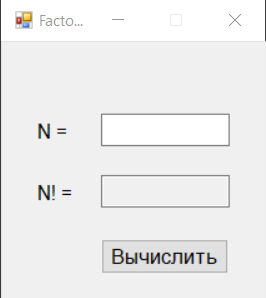
\includegraphics[width=0.4\linewidth]{lections/img/task1_launch1.png}
    \caption{Запуск программы}
    \label{task1_launch1}
\end{figure}
При вводе числа в поле ввода и нажатии на кнопку "Вычислить" (на рисунке \ref{task1_launch2})
\begin{figure}[H]
    \centering
    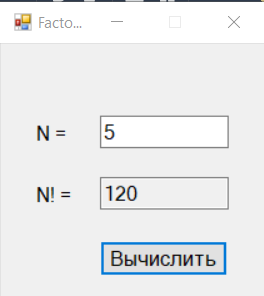
\includegraphics[width=0.4\linewidth]{lections/img/task1_launch2.png}
    \caption{Вычисление факториала}
    \label{task1_launch2}
\end{figure}
При попытке ввода не числа, программа выведет ошибку (на рисунке \ref{task1_launch3})
\begin{figure}[H]
    \centering
    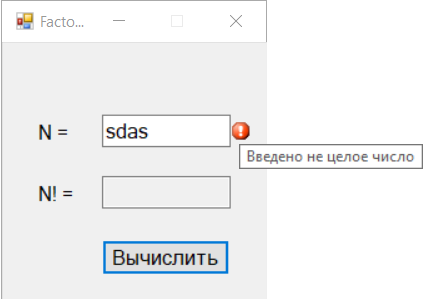
\includegraphics[width=0.4\linewidth]{lections/img/task1_launch3.png}
    \caption{Ошибка формата ввода}
    \label{task1_launch3}
\end{figure}
\subsection{Примеры исходного кода}

Код, выполняющийся при нажатии на кнопку "Вычислить".
\begin{minted}[style=bw,
 linenos=true,
 breaklines=true,
 numbersep=5pt,
 tabsize=2,
 fontsize=\small,
 bgcolor=white]{cpp}
private: System::Void solve_Click(System::Object^ sender, System::EventArgs^ e) {
	this->output->Text = "";
	errorProvider1->SetError(input, String::Empty);
	long long InputNumber;
	bool result = Int64::TryParse(this->input->Text, InputNumber); //переводим строку из TextBox число
	if (!result) { //dвели не число
		errorProvider1->SetError(input, "Введено не целое число");
	}
	else {//число
		if (InputNumber > 20) {
			this->output->Text = "Слишком большое число";
		}
		else {
			long long OutputNumber = fact(InputNumber);//результат
			if (OutputNumber == -1) { //отрицательное число
				errorProvider1->SetError(input, "Введено отрицательное число");
			}
			else { //все нормально
				this->output->Text = System::Convert::ToString(OutputNumber);//записываем в поле вывода
			}
		}
	}
}
\end{minted}
Другие фрагменты кода расположены в приложении \ref{app:factorial}.
\sectionbreak